\chapter{Sviluppo del software}
\section{Model-View-Controller}
Il Model-View-Controller (d'ora in poi MVC) è un pattern architetturale molto diffuso per la progettazione di sistemi software, in particolare di software basati sul paradigma di programmazione orientata agli oggetti.\\
\\
Il codice dell'applicazione viene quindi diviso in tre parti ben separate:
\begin{itemize}
    \item Model: codice che incapsula lo stato corrente dell'applicazione, ovvero i suoi dati.
    Può notificare la View quando si vengono a verificare cambiamenti nello stato dell'applicazione che portano ad aggiornamenti della View stessa.
    \item View: gestisce la parte grafica dell'applicazione e può richiedere dati al Model per aggiornarsi. Al verificarsi di eventi utente, inoltre, notifica il Controller.
    \item Controller: gestisce la logica dell'applicazione. Mappa gli eventi utente agli aggiornamenti dei modelli: al verificarsi di un certo evento, il Controller esegue l'aggiornamento (se necessario) sui dati del modello adatti.
\end{itemize}
Il controller può essere implementato seguendo diversi pattern, detti Controller Design:
\begin{itemize}
    \item page controller;
    \item front controller;
    \item intercepting filter;
    \item application controller.
\end{itemize}
La view può invece essere implementata seguendo i seguenti pattern, detti View Design:
\begin{itemize}
    \item template view;
    \item transform view;
    \item two-steps view.
\end{itemize}

\subsection{Controller Design}
I Controller Design sono i pattern che possono essere seguiti per l'implementazione del Controller.
\subsubsection{Page Controller}
In questo pattern, ogni pagina dell'applicazione ha un Controller associato. Di conseguenza, se il numero di pagine è elevato, il numero di Controller è elevato.
Il Controller associato a una certa pagina gestisce tutte le richieste provenienti da quella pagina.\\
\\
Il control flow di un Controller definito secondo questo pattern architetturale può essere riassunto come segue:
\begin{enumerate}
    \item a seguito di un'azione utente su una certa pagina, una View notifica il Controller associato alla pagina;
    \item il Controller analizza i parametri della richiesta e analizza la loro correttezza;
    \item il Controller richiama la logica corretta per la gestione della richiesta;
    \item il Controller sceglie la prossima pagina da mostrare;
    \item il Controller prepara i nuovi dati, che verranno mostrati nella prossima pagina;
    \item il Controller restituisce il controllo alla View da cui ha ricevuto la richiesta.
\end{enumerate}

\subsubsection{Front Controller}
Il pattern Front Controller permette di definire un unico Controller che riceve tutte le richieste, evitando quindi di implementare Controller multipli e di duplicarne il codice, come avviene invece in Page Controller. Una View può interagire con questo Controller solo usando specifiche operazioni, che vanno a definire un'interfaccia.\\
\\
In questo tipo di approccio, oltre al Controller, viene definita una classe astratta Comando,
che presenta un metodo virtuale Process.
Ogni operazione dell'interfaccia viene poi implementata come una classe concreta, figlia della classe astratta Comando, che effettua l'override del metodo Process: in questo metodo viene posta la funzionalità vera e propria dell'operazione.
A loro volta le classi possono essere organizzate in una gerarchia, in modo da riutilizzare codice all'interno di classi diverse.

Invocare un'operazione è quindi semplicemente una richiesta al Controller di eseguire la funzionalità espressa da una particolare classe concreta.\\
\\
Al crescere della dimensione dell'applicazione, il numero di operazioni (e quindi di classi concrete) deve aumentare: non deve infatti essere presente un'operazione monolitica che racchiude più funzionalità.

\subsubsection{Intercepting Filter}
Questo pattern è utilizzato, solitamente insieme al Front Controller, per eseguire codice su tutte le richieste di un certo tipo (ad esempio quelle provenienti da un determinato URL).

\begin{figure}[H]
    \centering
    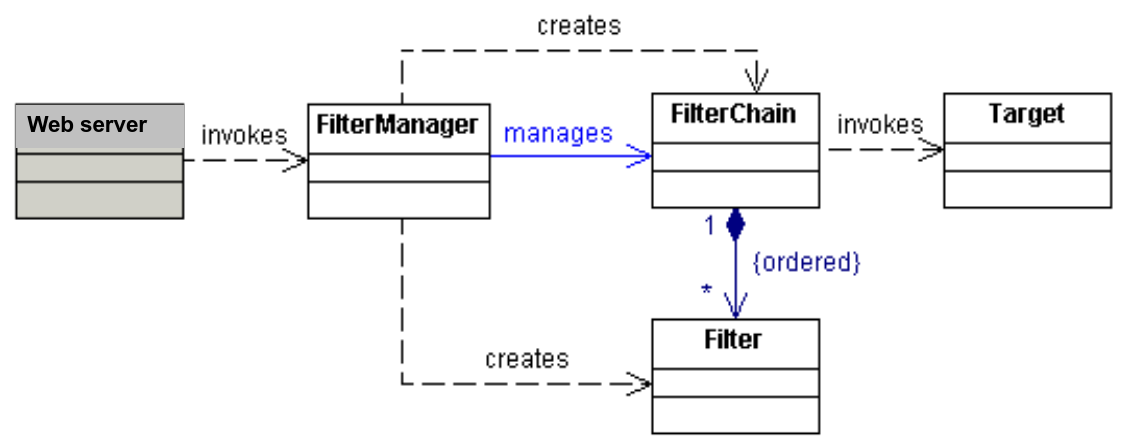
\includegraphics[width=1\linewidth]{images/intercepting_filter.png}
    \caption{Relazioni tra classi software in Intercepting Filter}
    \label{fig:intercepting_filter}
\end{figure}
Viene definito un Filter per ognuna delle funzionalità di Filtering. Ogni Filter è composto da una parte di pre-elaborazione e una di post-elaborazione. Non è però obbligatoria la presenza di entrambe: un filtro può infatti presentare solo una fase di pre-elaborazione o solo una fase di post-elaborazione.\\
\\
Una FilterChain raccoglie tutti i Filter che devono essere applicati a un certo tipo di richiesta: se viene ricevuta una richiesta che deve essere gestita con una particolare FilterChain, tutti le fasi di pre-elaborazione dei filtri presenti nella FilterChain vengono eseguite in ordine, per poi eseguire la logica di business corretta e infine eseguire tutte le post-elaborazioni, ma nell'ordine inverso rispetto all'ordine dei Filter all'interno della FilterChain.\\
\\
Un FilterManager raccoglie e gestisce tutte le possibili FilterChain, e si occupa di gestire una richiesta con la FilterChain corretta.
\begin{figure}[H]
    \centering
    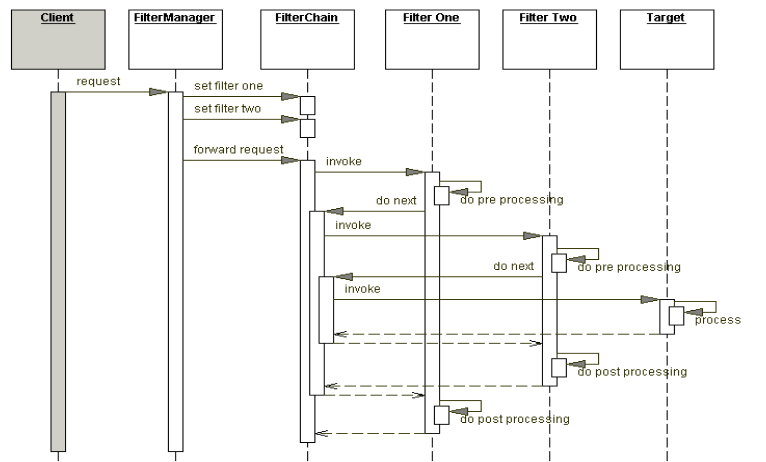
\includegraphics[width=1\linewidth]{images/filterchain_execution.png}
    \caption{Esempio di esecuzione dei filtri di una FilterChain}
    \label{fig:filterchain_execution}
\end{figure}


\subsection{View Design}
I View Design sono i pattern che è possibile seguire per implementare la View.

\subsubsection{Template View}
Il codice HTML di una pagina viene generato dinamicamente a partire da pagine template. Ogni pagina template è formata da una parte statica, ovvero codice HTML già specificato, e una parte dinamica, che genera altro codice HTML che andrà ad affiancarsi a quello già presente della parte statica.
La generazione della parte dinamica si basa sui dati contenuti nei modelli.
È solitamente usato congiuntamente a Page Controller.\\
\\
L'esecuzione della pagina dinamica può essere sia lato server che lato client: nel primo caso, il server genera completamente la pagina, e poi la invia al client; nel secondo caso, invece, il client riceve una pagina template, e procederà a eseguire richieste al Model lato server in modo da completare la pagina.

La scelta sul tipo di architettura (lato client o lato server) da adottare può basarsi sui seguenti criteri:
\begin{itemize}
    \item l'architettura lato server è più veloce nella costruzione della pagina completa se il numero di client è gestibile, altrimenti è consigliato gestire la costruzione della pagina lato client;
    \item l'architettura lato client permette di mostrare prima la pagina incompleta, ma richiede tempo per completarla;
    \item se i dati richiesti da una pagina cambiano spesso, allora è meglio utilizzare un'architettura lato client, in quanto permette di modificare solo piccole parti della pagina già presente sul client.
    L'architettura lato server richiederebbe infatti una rigenerazione dinamica dell'intera pagina, e il suo invio al client, a ogni modifica di un dato.
\end{itemize}

\subsubsection{Transform View}
In questo tipo di pattern, la View viene ottenuta tramite un processo di trasformazione: ogni dato di un Model viene infatti codificato in una stringa XML e una pagina viene generata combinando tutte le stringhe dei dati richiesti. Una pagina generata tramite Transform View è completamente dinamica: non sono infatti previste parti statiche.
\\
Quando una stringa XML viene richiesta, ovvero il relativo dato deve essere mostrato, essa viene passata a un classe Transformer, che raccoglie tutte le stringhe XML dei dati richiesti e genera la pagina.
La generazione della pagina da parte del Transformer può essere modificata usando regole di personalizzazione: a ogni dato possono essere associate più regole, che permettono di modificarne il rendering.
Le regole sono specificate con un apposito linguaggio di trasformazione.\\
\\
Un possibile svantaggio che presente questo approccio è che non è possibile visualizzare la pagina, nemmeno incompleta, prima che siano state elaborate tutte le regole e generata l'intera pagina completa.
Inoltre, essendo la pagina risultante dipendente dai dati da cui è costruita, il testing può complicarsi. Si semplifica invece il testing delle regole di trasformazione, in quanto semplici stringhe.

\subsubsection{Two-step View}
DA FINIRE

\subsection{Spring MVC}
DA FINIRE